\chapter{Production of English [Cs] clusters by Brazilian speakers: effects of orthography, phonological environment and task type}
\label{ch:wellingtonara4}
\chapterauthor[1]{Wellington Araujo Mendes Junior}
\begin{affils}
\chapteraffil[1]{Federal University of Minas Gerais}
\end{affils}

This study examines the effects of orthography, phonological environment
and task type in the production of English {[}Cs{]} clusters by
Brazilian Portuguese (BP) speakers. Two orthographic patterns were
examined for English nouns whose plural is pronounced as a (stop +
sibilant) cluster. One of the patterns presents two consonants
word-finally - \emph{cups}, \emph{cats}, \emph{ducks} - whereas the
other one presents a silent vowel \textless{}e\textgreater{} between two
consonants: \emph{grapes}, \emph{plates}, \emph{cakes}. The goal was to
assess whether these different orthographic patterns would trigger the
production of an epenthetic vowel. Additionally, it was assessed whether
different phonological environments would influence the voicing property
of the final sibilant. As it is known, word-final English sibilants are
prone to progressive assimilation (e.g. \emph{cups} {[}kʌps{]},
\emph{bags} {[}bæɡz{]}), rather than regressive assimilation -- as it
occurs in BP (\emph{mês} {[}mes{]}, \emph{mês} \emph{anterior} {[}mez
ə̃.te.ɾi.ˈoɾ{]}). An experiment was designed to test the production of
{[}Cs{]} clusters in English nouns and in BP forms undergoing sound
change. Harmonics-to-noise ratio (HNR) was used to measure sibilant
voicing, whereas the presence of epenthetic vowels was assessed
categorically. Results showed that English learners are more likely to
pronounce a vowel when the orthographic pattern is
\textless{}Ces\textgreater{} rather than \textless{}Cs\textgreater{}, and
this occurs regardless of the visual presentation of the words.
Moreover, HNR rates showed that fully voiced sibilants tend to occur in
L2 English when the consonant is both preceded and followed by a vowel.
These findings are discussed in light of the Exemplar Model in L2
Phonology (EML2P) \citep{guimaraes2021,mendesjr2022}. The
analysis based on the EML2P showed that robust patterns from the L1 are
adopted in L2, including fine phonetic detail that reflects subphonemic
properties.

\section{Introduction}
Traditional phonological models assume that English plural suffixes and
third person singular present forms are subject to a phonological rule.The
underlying representation for regular plural and
3\textsuperscript{rd} person singular present is assumed to be /z/ \citep{hayes2011}.
A progressive assimilation rule predicts that if a vowel
or a voiced consonant precedes /z/, the output is {[}z{]}, as in\emph{dogs}
{[}dɒɡz{]}, \emph{trees} {[}triːz{]} and \emph{pies}
{[}paɪz{]}. If a voiceless consonant precedes /z/, it surfaces as{[}s{]}, as in
\emph{cups} {[}kʌps{]}, \emph{cats} {[}kæts{]} and
\emph{ducks} {[}dʌks{]}. Finally, if an alveolar fricative or anaffricate
precede the sibilant, the outcome is {[}ɪz{]}, as in\emph{buses} {[}bʌsɪz{]},
\emph{quizzes} {[}kwɪzɪz{]} and \emph{watches}{[}wɒtʃɪz{]}. However, when we
consider the orthography of English
plural forms, two possible spellings are associated with theaforementioned
sound patterns. Nouns can either end in a consonant
followed by the letter \textless s\textgreater, as in \emph{books}
and\emph{jobs} or the by letters \textless es\textgreater, as in
\emph{cakes} and \emph{cubes.} Brazilian Portuguese, on the other hand,
presents mainly the \textless Ces\textgreater{} pattern, as it occurs
in\emph{cheques }and\emph{ clubes}, whereas only some few nouns present
the \textless Cs\textgreater{} pattern: \emph{biceps},
\emph{forceps},\emph{volts}.

As a consequence of an ongoing sound change, word-final {[}Cs{]}
clusters\footnote{ For the purpose of the present discussion, we refer  to
{[}Cs{]} as any (consonant + sibilant) sequence. However, as it
will be discussed later, the sibilant may be either voiced or  voiceless.}
are currently very productive some Brazilian Portuguese
plural forms: \emph{crepes}, \emph{potes}, \emph{cheques} \citep{soares2016}. The
alternation between {[}Cs{]} \textasciitilde{} {[}Cis{]}
word-finally in BP follows from the reduction and eventual loss ofunstressed
high front vowels when flanked between a consonant and a
word-final sibilant. It seems that such alternation also applies toplural forms
produced by Brazilian speakers of L2 English, as in\emph{cakes} {[}keɪks{]}
\textasciitilde{} {[}'keɪ.kis{]}.

This paper intends to investigate {[}Cs{]} clusters in English regular
plural forms (e.g. \emph{cups} {[}kʌps{]}, \emph{grapes} {[}ɡreɪps{]})produced
by Brazilian speakers of L2 English in an attempt to address
the question of whether an ongoing sound change from the L1 plays a rolein L2
learning. Additionally, we aim to assess how orthographic and
phonological representations are related. Studies on the relationshipbetween
orthography and phonology have increased in recent years
\citep{rafat2015,hamann2017,zhou2021}.
The main research questions in this topic aim to explain how
L2 learners mediate the relationship between the already knownphonological and
orthographical knowledge from the L1 in order to buildan L2. Thus, an important
question we pose is whether differentorthographic patterns trigger different
pronunciations of {[}Cs{]}
clusters in L2 English.

This paper is organized as follows. The next section reviews studies on
the production of English {[}Cs{]} clusters by Brazilian speakers. Thethird
section describes the methodology adopted in this study. The
fourth section discusses our findings and is followed by theconclusions.



\section{Production of English {[}Cs{]} clusters by Brazilian speakers}
Several works have addressed the relationship between orthography and
the pronunciation of L2 English forms by Brazilian speakers. One of themain
concerns have been to assess whether the presence of an epenthetic
vowel in L2 English is influenced by a letter corresponding to a
vowel. \citet{delatorre2006} investigated the
production of English {[}Cs{]} clusters that occur in past andparticiple forms
by Brazilian speakers of L2 English (e.g. \emph{moved}
and \emph{robbed}). Two epenthetic vowels were attested: one epentheticvowel
breaks up the word-internal consonant cluster and the other one
prevents word-final consonants, as in
\emph{asked}{[}'as.k\textbf{e}.dʒ\textbf{i}{]} and
\emph{saved}{[}'seɪ.v\textbf{e}.dʒ\textbf{i}{]}. \citet{delatorre2006} claimed that
theorthographic input, which was present in a reading task, favored higher
rates of an epenthetic vowel, as opposed to a free speech task, whichdid not
present any orthographic stimulus. Therefore, she argued that
the orthographic input favored the presence of epenthetic vowels in
the pronunciation of L2 English by Brazilian speakers.

Although she did not focus on the
production of {[}Cs{]} clusters, \citet{silveira2007} also investigated
the production of word-final epenthesis in Brazilian speakers of L2 English.
She compared words whose final letter was a consonant (e.g. mad{[}mæd{]}) to
words whose final letter was a silent ⟨e⟩ (e.g.
\emph{made} {[}meɪd{]}). Her results showed that words ending in asilent ⟨e⟩
presented higher rates of epenthesis than words that ended in
a consonantal letter. Akin to \citet{delatorre2006}, the results of \citet{silveira2007}
showed that a reading task favored higher rates of epenthetic
vowels than a free speech task, indicating that orthographic input (and the task
type) contributed to the production of an epenthetic vowel.

Another case of epenthetic vowels reported in the literature involves
word-final consonant and sibilant sequences, {[}Cs{]}, which typically appear in
regular plural and 3\textsuperscript{rd} person singular
present forms in English. It is known that Brazilian speakers of L2English
tended to insert an epenthetic vowel between two word-final
consonants, as it occurs, for example, in \emph{cakes}
{[}keɪks{]}\textasciitilde{} {[}'keɪ.k\textbf{i}s{]} \citep{cristofato2011}.
Interestingly, works that considered 3\textsuperscript{rd} person singular
present and regular plural forms in English spoken by Brazilian
speakers did not account for an epenthetic vowel. They were rather concerned
with voice agreement.

\citet{zanfra2013} studied sibilant voicingin L2 English by Brazilian speakers.
Although her focus was not
specifically on plural forms, her results shed some light on the
current discussion. The author tested whether the BP voicing assimilation rule
involving adjacent segments in word boundaries would apply in L2
English learners' productions. Her results showed that sibilants tended to be
voiced when followed by a voiced consonant (e.g. \emph{The}\emph{hou\textbf{s}e
\textbf{b}ackyard} \emph{is huge}) or by a vowel
(e.g. \emph{The} \emph{mou\textbf{s}e \textbf{I}} \emph{saw is
white}).Conversely, a sibilant was voiceless when the following context was
a pause (e.g. \emph{I won't go if he goe\textbf{s}}.) or a voiceless consonant
(e.g. \emph{The\textbf{s}e pancakes} \emph{are great}). \citet{zanfra2013}
suggested that Brazilian speakers of L2 English speakers transfer the BP
regressive assimilation rule into their L2 English.

\citet{fragozo2017} investigated the
voicing of sibilants in English regular plural forms and 3\textsuperscript{rd}
person singular presented by Brazilian speakers of
L2 English. She assessed the extents to which a sibilant would be voiced after a
voiced consonant, as in \emph{dogs} or \emph{clubs}, which would
reflect the acquisition of a progressive assimilation rule from English.
\citet{fragozo2017} also examined words in context to verify if the
regressive assimilation rule, which applies to BP, would be transferred to L2
English. She found that voiced sibilants tended to follow the
regressive assimilation rule from BP, whereas the English
progressive assimilation rule had a very low rate in her data (0.6\%). She
argues that the low rates of voiced sibilants {[}z{]} in L2 English by Brazilian
speakers follows from the fact that these consonants are only
partially voiced in English. Data from her control group of native speakers
presented 44\% of expected voiced sibilants. Thus, as sibilants
are partially voiced in English, they would not be accessible in L2 English.

\citett{zanfra2013,fragozo2017} both investigated voicing agreement
within a rule-based approach where there would be a competition between a
regressive assimilation rule from BP and a progressive assimilation
rule from English. A question that arises from this assumption is whether a rule
that is transferred from the L1 to the L2 could change as
time goes by. Another issue which is polemic lies on the role played
by orthography, as in hou\textless se\textgreater{}\emph{ }or\emph{}bu\textless s\textgreater{} 
\citep{zanfra2013}. Orthography cannot bemodelled
within a rule-based approach as it is not part of Grammar.
Furthermore, the rule-based approach adopted by \citett{zanfra2013,fragozo2017}
neglected the role played by an epenthetic vowel that may intervene between the
two word-final consonants, as in \emph{cakes}{[}keɪks{]} \textasciitilde{}
{[}'keɪ.k\textbf{i}s{]}. Additionally,
they did not account for the gradience of sibilant voicing.

Unlike previous works which adopt rule-based approaches, this paper
models L2 phonology within an Exemplar Model by considering
representation robustness and the role of fine phonetic detail in
shaping mental representations. Within this proposal, orthography is
modelled as part of the linguistic knowledge of literate speakers and
sound patterns display a great range of variability and gradience.


\section{Methodology}
A set of 36 plural nouns ending in a sequence of (stop + sibilant) were
considered in BP. These words present a single orthographic pattern:
\textless Ces\textgreater, as in \emph{cheques} {[}ʃɛks{]}
\textasciitilde{} {[}'ʃɛ.kis{]} `cheques'. For the L2 English case
study, a set of 36 words were selected, where 15 words display the
orthographic pattern \textless Ces\textgreater, as in \emph{grapes}
{[}ɡreɪps{]}, and the other 21 words display the orthographic pattern
\textless Cs\textgreater, as in \emph{maps} {[}mӕps{]}.

The experiment comprised two tasks. The first one consisted of a
picture-counting task in which participants were asked to count and name
the items shown in the pictures. Short carrier sentences that did not
include orthographic stimuli of the target words were given. The second
trial consisted of a reading task. Initially, participants were asked to
read 72 BP sentences aloud. Alike the picture-counting task, BP nouns in
the reading task were followed by either a vowel or a voiceless
consonant. On the other hand, L2 English nouns were followed by either a
vowel or a pause. The overall number of syllables was controlled for
both languages: 4 in English and 12 in BP, considering the deletion of
the {[}i{]} vowel. Sentence-level intonation and the morphological class
of each word were also controlled.

A group of six Brazilians studying at the Federal Center for
Technological Education of Minas Gerais, in the city of Araxá,
participated in this study\footnote{This research has been approved by
the ethics committee from the Universidade Federal de Minas Gerais,
reference number: CAAE: 15116119.9.0000.5149.}. All participants were
high school students who had been taking English classes as part of the
school's curriculum for about~one year. The group consisted of 3~males
and~3~females and their ages ranged from 15 to 17. All participants
displayed either B1 or B2 proficiency levels (intermediate learners) of
the Common European Framework of Reference for Languages.

Due to the recent COVID-19 pandemic, all interactions were performed
remotely. Experiments were recorded with the \emph{Open Broadcaster
Software Studio}~at 48 kHz sampling rate. The obtained recordings were
converted into WAVEform audio format by the software~\emph{Adobe
Premiere 2020}, which was able to maintain the same sampling rate as the
original files. The average time to complete the experiment was 45 minutes. 
A total of 648 tokens were collected for the L2 English study.
For the BP study, 432 tokens were collected. Samples were edited and
manually annotated using Praat~TextGrids \citep{boersma2020}.

Besides assessing the presence or absence of a vowel between {[}Cs{]}
clusters, this research also considered the voice quality of word-final
sibilants. In BP, only voiceless sibilants occur word-finally, unless a
vowel follows it, to which a voiced sibilant occurs. In English, voiced
and voiceless sibilants occur word-finally. When a vowel follows the
sibilant, the voice quality remains as it formerly was (rather that
changing as it occurs in BP). We posited that word-final voiceless
sibilants would be favored in L2 English, as it is the more robust
pattern in L1. We also posited that a voiced sibilant occurs at higher
rates in an intervocalic position: {[}Cis{]} followed by a word-initial
vowel.

Voicing was measured under Harmonics-to-noise ratio. Each token was
extracted to a separate sound object and a harmonicity object was
created, from which the mean harmonicity was calculated, hereafter the
HNR. The details of its calculation can be found in \citet{Boersma93}.
Harmonicity would seem to be a good measurement of voicing since vocal
cord vibration produces ``a complex periodic wave'' \citep[p.~63]{johnson1997}. 
Based on the discussion from Praat's manual, higher values of HNR
should correspond with higher voicing rates.



\section{Results}

Consider Figure \ref{wel-fig1}, which shows the rates of {[}Cs{]} in regular plural
forms in BP and L2 English.

\begin{figure}[h]
\centering
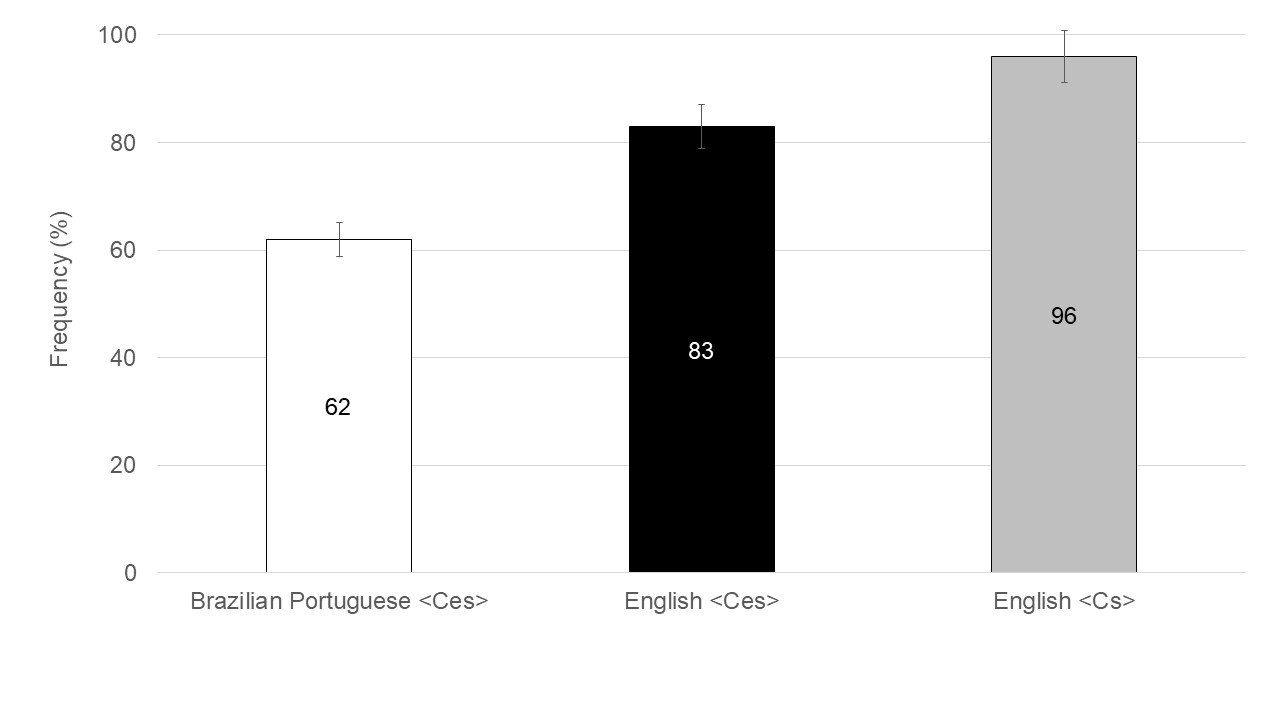
\includegraphics[width=\linewidth]{imgs/wellingfig01.png}
\caption{{[}Cs{]} rates by orthographic patterns.}
\label{wel-fig1}
\end{figure}

The leftmost column shows that regular plural forms in BP, whose
orthography is \textless Ces\textgreater, presented 62\% of a consonant
followed by a sibilant: {[}Cs{]}. That means that when a letter
\textless e\textgreater{} appears in the orthography of BP plural forms,
a vowel is manifested in 38\% of the cases. The two rightmost columns
report data from English spoken by Brazilian speakers. When the
orthography in the plural form is \textless Ces\textgreater, a consonant
followed by a sibilant {[}Cs{]} occurred in 83\% of the cases, whereas
in the cases where the orthography was \textless Cs\textgreater, a
consonant followed by a sibilant occurred in 96\% of the productions.
This result shows that the pronunciation of {[}Cs{]} is more recurrent
when the orthography is \textless Cs\textgreater{} than when the
orthography is \textless Ces\textgreater{} in regular plural forms in
English. In other words, a vowel will appear at higher rates when the
orthographic pattern is \textless Ces\textgreater{} than when it is
\textless Cs\textgreater. Thus, it is more likely that a plural form as
\emph{tapes} will have a vowel pronounced between the last two
consonants than a plural form as \emph{maps}. The difference between the
data presented in the two rightmost columns is statistically significant
for the orthographic patterns (χ2 = 36.113, df = 1, p \textless{} 0.01).
The explanation for such difference lies in the different orthographic
patterns.

We also considered whether different tasks could favor the production of
an epenthetic vowel. According to \citett{delatorre2006,silveira2007},
visual input favors such non-target productions. In our experiment, the
picture-counting task had no orthographic visual input, whereas
orthography was available in the reading task. If \citett{delatorre2006,silveira2007} 
are correct, then we expect that vowels would occur at
higher rates in the reading task than in the picture-counting task in
our experiment. However, no statistically significant differences were
found between the picture-counting task and the reading task (χ2 = 0.66,
df = 1, p-value = 0.41). This shows that it is the orthographic pattern
rather the type of task that favors a vowel to occur in L2 English. Our
claim is that once speakers are literate, orthography is part of their
grammar, i.e., it has a permanent impact on mental representations. The
EML2P model adopted in the current paper differs from \citett{delatorre2006,silveira2007,zanfra2013}
rule-based approach mainly by
assuming that orthography is part of linguistic knowledge and not
external to it.

Another research question we posited regarded the voice quality of the
word-final sibilant in {[}Cs{]} and {[}Cis{]}. This was the main issue
considered by \citet{zanfra2013,fragozo2017} within a rule-based
approach. Their analysis claimed that voicing in L2 English did not
achieve the target rates due to constraints of BP distribution of
sibilants and regressive assimilation. BP only presents voiceless
sibilants word-finally. However, across word-boundaries, BP sibilants
are voiced when followed by a voiced consonant or a vowel: \emph{mês}
{[}mes{]} `month', \emph{mês bonito} {[}mez ˈbo.ni.tu{]} `beautiful
month', \emph{mês anterior} {[}mez ə̃.te.ɾi.ˈoɾ{]} `previous month'. In
this paper, we offer an alternative view to the preceding rule-based
approaches. Within the scope of the EML2P, it is suggested that
generalizations from an ongoing sound change in BP phonology are
transferred into L2 English, where phonetic detail plays an important
role in shaping mental representations. Consider Figure \ref{wel-fig2}.


\begin{figure}[h]
\centering
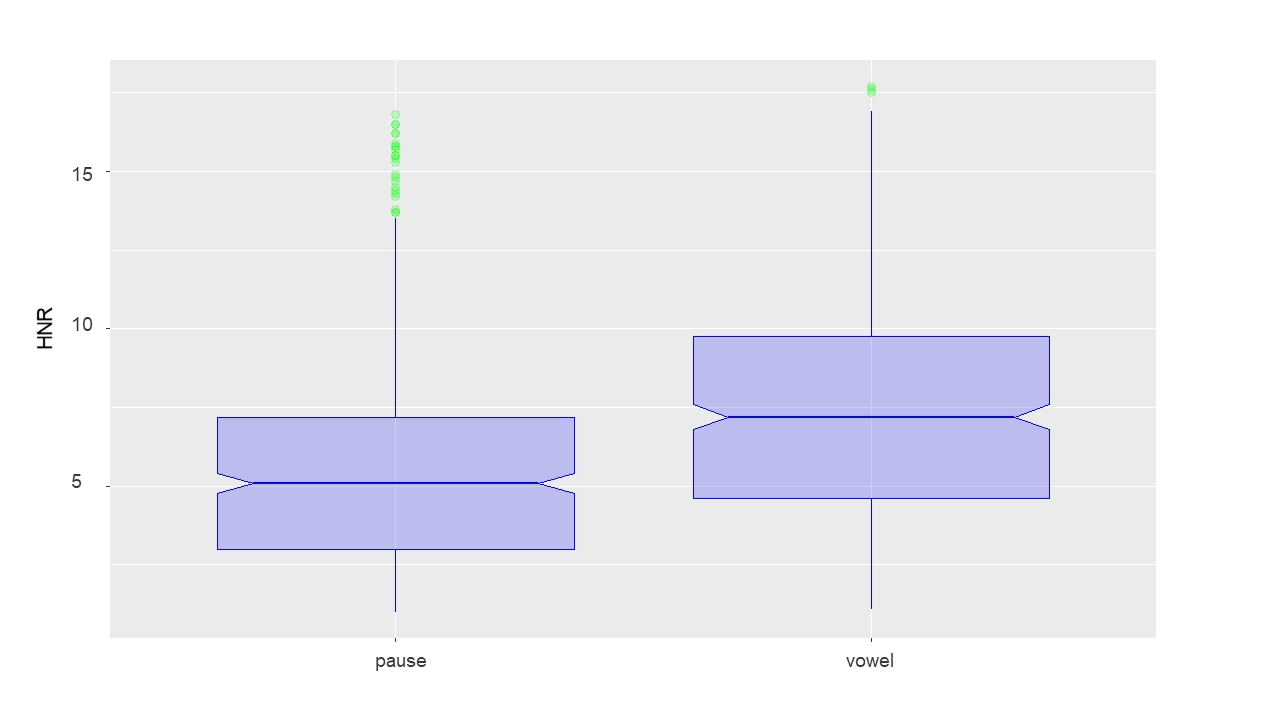
\includegraphics[width=\linewidth]{imgs/wellingfig02.png}
\caption{HNR per following phonetic environment in L2 English.}
\label{wel-fig2}
\end{figure}

The boxplots in Figure \ref{wel-fig2} show harmonics-to-noise ratio per following
phonetic environment in L2 English. We can see that when the sibilant is
followed by a pause, it tends to be unvoiced, with HNR rates at around 5
decibels. Conversely, when the sibilant is followed by a vowel, voicing
rates are higher. T-test results show that there is a significant
difference in HNR between both following phonetic environments (t = -8.8153, 
df = 821.37, p-value \textless{} 0,01). However, even though
such environments seem to influence voicing rates of the final sibilant,
these rates are still lower when compared to English target forms. To
put it another way, nouns that should be pronounced with a word-final
voiced sibilant present more unexpected voiceless sibilants than voiced
ones. This can be accounted by the fact that only voiceless sibilants
occur word-finally in BP. Learners are likely unaware of the fact the
{[}z{]} should be voiced in accordance with the voice property of the
preceding segment. Now consider Figure \ref{wel-fig3}.

\begin{figure}[h]
\centering
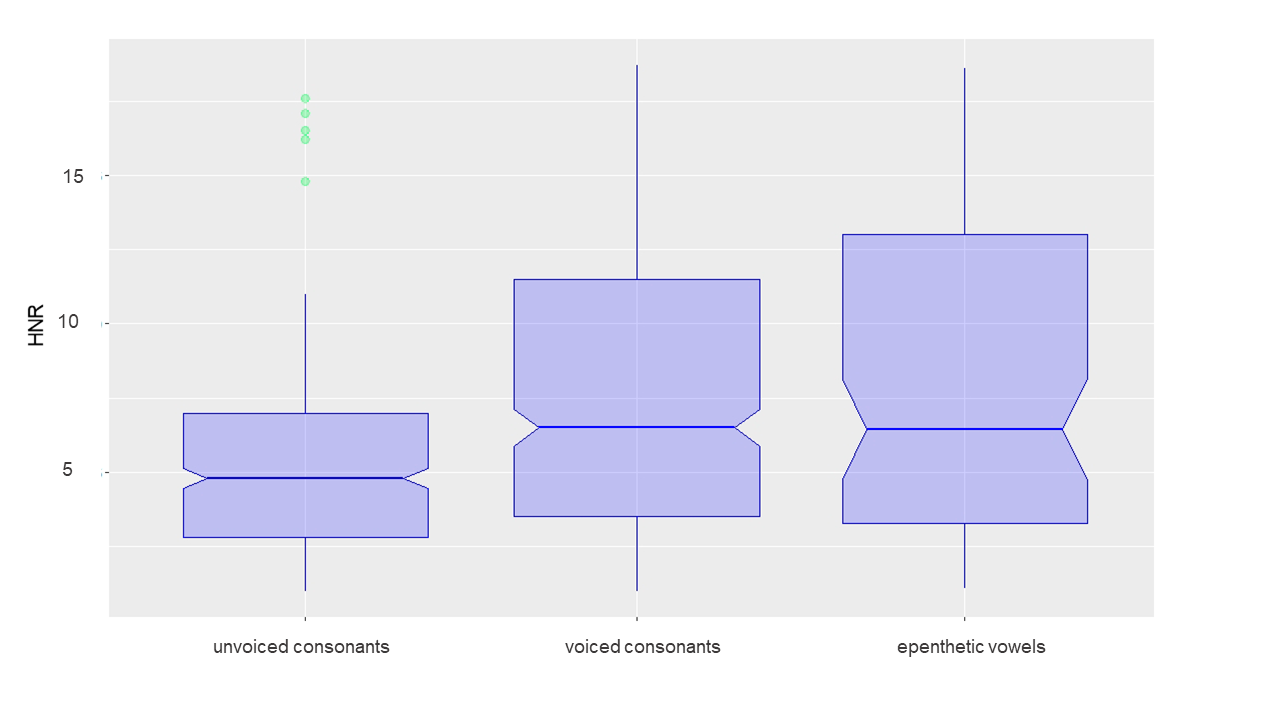
\includegraphics[width=\linewidth]{imgs/wellingfig03.png}
\caption{HNR per preceding phonetic environment in L2 English.}
\label{wel-fig3}
\end{figure}

The boxplots in Figure \ref{wel-fig3} show harmonics-to-noise ratio per preceding
phonetic environment in L2 English. Data is comprised of sibilants
preceded either by an unvoiced consonant, a voiced consonant or an
epenthetic vowel. At first sight, we can see the HNR rates are somewhat
lower when the sibilant is preceded by an unvoiced consonant, and higher
rates occur when the sibilant is followed by voiced consonants and
epenthetic vowels. An analysis of variance (ANOVA) on these scores
yielded significant variation among conditions: F(2,858)=59.99, 
p\textless{} 0.001. A post-hoc Tukey test showed that the group comprised
of unvoiced consonants differed significantly at p \textless{} 0.05; the
voiced consonants group was not significantly different from the
epenthetic vowels group. This result suggests that epenthetic vowels
contribute to higher rates of voicing as much as other voiced segments
in L2 English. Finally, an interaction between both preceding and
following phonetic environments was attested {[}F(2,858)=7.797, p
\textless{} 0.001{]}.

Our results throw some light on the line of research carried out by
\citett{zanfra2013,fragozo2017}, who investigated the sibilant voicing
followed by a vowel within rule-based approaches. We account for the
fact that low HNR (which reflect voiceless sibilants) is recurrent in
regular plural forms in L2 English, as {[}s{]} is the most robust
exemplar in word-final position in BP. We also account for the fact that
the pattern {[}Cis{]} favors a voiced sibilant in L2 English, as voiced
sibilants are favored in similar contexts in BP (i.e., intervocalically). 
This indicates that L1 exemplar patterns, which
reflect subphonemic information, are adopted in the L2. Finally, our
analysis explains why {[}z{]} presents a low rate of production in L2
English spoken by Brazilian speakers: it is an emerging pattern in the
L2, since it has no exemplars from the L1, at least not in word-final
position. It will be through experience that these exemplars will become
robust and more recurrent.



\section{Conclusions}
The aim of this paper was to investigate {[}Cs{]} clusters in English by
Brazilian speakers. Its main contribution was to assess the role of
orthography, phonological environment and task type not only on the
production of epenthetic vowels, but also on the voicing property of the
final sibilant. It also considered the role played by the {[}Cs{]}
\textasciitilde{} {[}Cis{]} ongoing sound change from BP into L2
English. Results showed that the orthographic pattern
\textless Ces\textgreater{} favors the production of an epenthetic vowel
at higher rates that the \textless Cs\textgreater{} pattern. As for the
task type, it was shown that it was not the visual access to
orthographic forms that triggered a vowel to occur, but rather the
orthographic patterns.

It was also shown that HNR is strongly influenced by
phonetic/phonological environments, including preceding epenthetic
vowels, which had not been accounted for in previous studies. We can
assume that {[}z{]} poses a challenge to Brazilian speakers of L2
English due to the fact that it still has no exemplars from L1 in
word-final position.

Concerning the role played by the BP ongoing sound change involving the
{[}Cs{]} \textasciitilde{} {[}Cis{]} alternation, it was shown that
robust patterns from the L1 are adopted in L2, including fine phonetic
detail that reflects subphonemic properties. This sheds light to the
fact that learners not only transfer sounds to the L2, but also
phonological behaviors in which such sounds are subject to (as seen with
how L2 voicing/HNR is influenced by L1 phonological patterns). We can
assume, thus, that better generalizations are posited when the
production of {[}Cs{]} clusters is assessed globally, rather than
accounting for epenthesis and voicing agreement as separate, unrelated
phenomena.


\bibliographystyle{plainnat}
\bibliography{wellingtonara4.bib}


